\setcounter{step}{0}
%------------------------------------------
% information doc
\subsection{Fake kekse ku káve}
\PrepTime{15}
\CookingTime{10-15}
\CookingTempe{180}
\TypeCooking{Pečenie}
\NbPerson{4}
\Image{0 0 430 430}{images/florentin} %style 2
%------------------------------------------

\begin{ingredient}
%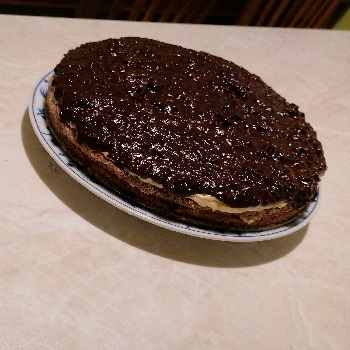
\includegraphics[height=5.5cm]{images/daim}
\def\portions{4}%
\textbf{{\normalsize Ingrediencie (\portions porcie):}}
%\vspace{0.5cm}
\begin{main}
	\item 125g maslo
	\item 125g cukor
	\item 2-3PL med
	\item 250g hladná múka
	\item štipka soli
	\item kypriaci prášok
\end{main}
\end{ingredient}
\begin{recipe}
\textbf{{\normalsize Príprava:}}
\begin{enumerate}


\item{Zmäknuté maslo vyšľahať s cukrom a štipkou soli}
\item{pridať múku s kypriacim práškom a med}
\item{Vyhnietiť do jemnej hmoty}	
\item{Nechať aspoň hodinu odpočinúť v chladničke}
\item{Vyvaľkať a vyťapkať z neho placky}
\item{Dať piecť do rúry}

\end{enumerate}
\end{recipe}

\begin{notes}

\end{notes}
\clearpage	